\documentclass{beamer}
\usetheme{metropolis}
\usepackage{graphicx}
\usepackage{subcaption}
\usepackage{hyperref}
\usepackage{tcolorbox}
\title{Algebra-Based Physics-1: Mechanics (PHYS135A-01): Week 8}
\date{October 23rd - October 27th, 2017}
\author{Jordan Hanson}
\institute{Whittier College Department of Physics and Astronomy}

\begin{document}
\maketitle

\section{Week 7 Review}

\begin{frame}{Week 7 Summary}
\begin{enumerate}
\item \alert{Work} has a scientifically precise definition
\item Kinetic Energy and the \alert{Work-Energy Theorem}
\item Gravitational potential energy
\item Definition of a \textbf{conservative force} and potential energy
\item Power and the human body
\end{enumerate}
\end{frame}

\section{Week 7 Review Problem}

\begin{frame}{Week 7 Review Problem}
\small
The Crab Nebula is the remnant of a \textit{\textbf{supernova}} that occurred in in A.D. 1054.  It is a pulsar that emits radio waves and gamma photons.  At peak radiation, a typical supernova yields $5\times 10^{37}$ Watts in power.  Today, the Crab Nebula yields $10^{28}$ Watts in power.  Since today's power there is so much smaller, let's assume that all of the energy emitted in by The Crab in the past thousand years is equivalent to the peak power ($5\times 10^{37}$ Watts) yielded over two weeks of time.  How much energy is this?
\begin{itemize}
\item A: $6\times 10^{42}$ J
\item B: $6\times 10^{43}$ J
\item C: $6\times 10^{44}$ J
\item D: $6\times 10^{45}$ J
\end{itemize}
\end{frame}

\section{Week 8 Summary}

\begin{frame}{Week 8 Summary}
\begin{enumerate}
\item Definition of \alert{\textbf{momentum}}
\item \alert{\textbf{\textit{Conservation of momentum}}}
\begin{itemize}
\item The proof and the assumptions
\item Examples
\end{itemize}
\item \alert{\textbf{\textit{Classification of collisions}}}
\begin{itemize}
\item Elastic
\item Inelastic
\item $1 \rightarrow 1$, $1 \rightarrow n$, $n \rightarrow 1$, $n \rightarrow n$
\item \textbf{Lab activity}
\end{itemize}
\item \textbf{Momentum in multiple dimensions}
\item \textbf{Center of mass}
\begin{itemize}
\item Derivation of $\vec{F}_{\rm Net} = \frac{d\vec{P}_{\rm CM}}{dt}$
\item Center of mass motion
\end{itemize}
\end{enumerate}
\end{frame}

\section{Definition of Momentum}

\begin{frame}{Definition of momentum}
\textit{Ready to jump down the rabbit hole?  Good.}  Momentum is defined as follows: \\ \vspace{1cm}
\begin{tcolorbox}[colback=white,colframe=red!40!blue,title=Definition of Momentum]
\alert{A particle of mass $m$ and velocity $\vec{v}$ has the vector \textit{momentum}:} \\ \\
\alert{$\vec{p} = m\vec{v}$}
\end{tcolorbox}
\end{frame}

\begin{frame}{Definition of momentum}
There is a corollary: \\ \vspace{1cm}
\begin{tcolorbox}[colback=white,colframe=red!40!blue,title=Newton's Second Law with momentum]
\alert{If a particle has acceleration $\vec{a} = \frac{d\vec{v}}{dt}$, then} \\ \\
\alert{$\vec{F}_{\rm Net} = \frac{d\vec{p}}{dt}$}
\end{tcolorbox}
\end{frame}

\begin{frame}{Definition of momentum}
An object that has a small mass and an object that has a large mass have the same momentum. Which mass has the largest kinetic energy?
\begin{itemize}
\item A: The one with the small mass
\item B: The one with the large mass
\item C: If the momentum is the same the kinetic energy is the same
\item D: Cannot determine the answer
\end{itemize}
\end{frame}

\begin{frame}{Definition of momentum}
An object that has a small mass and an object that has a large mass have the same kinetic energy. Which mass has the largest momentum?
\begin{itemize}
\item A: The one with the small mass
\item B: The one with the large mass
\item C: If the momentum is the same the kinetic energy is the same
\item D: Cannot determine the answer
\end{itemize}
\end{frame}

\begin{frame}{Definition of momentum}
The unit of linear momentum is kg m/s.  Suppose that a raindrop reaches a terminal velocity of 10 m/s, and the density of water is 1 gram per cm$^3$.  If a 1 cm$^3$ water droplet reaches terminal velocity, what is the momentum of the droplet?
\begin{itemize}
\item A: $10^{-3}$ kg m/s
\item B: $10^{-2}$ kg m/s
\item C: $10^{-1}$ kg m/s
\item D: $1$ kg m/s
\end{itemize}
\end{frame}

\begin{frame}{Definition of momentum}
An small meteor has a mass of $10^{3}$ kg and a velocity of 10 km/s as it enters Earth's atmosphere.  What is the initial momentum?
\begin{itemize}
\item A: $10^{7}$ kg m/s
\item B: $10^{6}$ kg m/s
\item C: $10^{5}$ kg m/s
\item D: $10^{4}$ kg m/s
\end{itemize}
\end{frame}

\begin{frame}{Definition of momentum}
If it drag of the atmosphere brings the meteor particles to rest, the final momentum is zero.  If the average net force on the system is $F_{\rm Net} = \frac{\Delta p}{\Delta t}$, and the meteorite exists for 1 second, what is the average force on the meteorite?
\begin{itemize}
\item A: $10^{7}$ N
\item B: $-10^{7}$ N
\item C: $10^{6}$ N
\item D: $-10^{6}$ N
\end{itemize}
\end{frame}

\section{Conservation of Momentum}

\begin{frame}{Conservation of Momentum}
\textit{...continuing to fall down the rabbit hole...} \\ \vspace{1cm}
\begin{tcolorbox}[colback=white,colframe=red!40!blue,title=Conservation of Momentum]
\alert{The momentum of a system of $N$ particles undergoing no external forces is conserved.} \\ \\
\alert{$\frac{d\vec{P}}{dt}=0$}
\end{tcolorbox}
\end{frame}

\begin{frame}{Conservation of Momentum}
Suppose two objects with momenta $\vec{p}_{\rm 1} = m_{\rm 1}\vec{v}_{\rm 1}$ and $\vec{p}_{\rm 2} = m_{\rm 2}\vec{v}_{\rm 2}$ collide. The new momenta after the collision are $\vec{p}'_{\rm 1} = m_{\rm 1}\vec{v}'_{\rm 1}$ and $\vec{p}'_{\rm 2} = m_{\rm 2}\vec{v}'_{\rm 2}$.  If $m_{\rm 2} = 2 m_{\rm 1}$ and $\vec{v}_{\rm 1} = 2\vec{v}_{\rm 2}$, and $\vec{v}'_{\rm 2}$ is observed to equal $\vec{v}_{\rm 1}$, what is $\vec{v}'_{\rm 1}$? \\ \vspace{1cm}
\textbf{Solve together in groups on boards.}
\end{frame}

\begin{frame}{Conservation of Momentum}
\small
The proof of conservation of momentum is the combination of two concepts: \alert{\textbf{Newton's 3rd Law}} and \alert{\textbf{Newton's 2nd Law}}.  The net forces on two particles by Newton's 3rd Law are 
\begin{equation}
\vec{F}_{\rm 21} = -\vec{F}_{\rm 12}
\end{equation}
Substituting Newton's 2nd Law for the forces,
\begin{equation}
m_{\rm 1} \vec{a}_{\rm 1} = -m_{\rm 2}\vec{a}_{\rm 2}
\end{equation}
Acceleration is defined as the change in velocity, implying
\begin{align}
m_{\rm 1} \frac{d\vec{v}_{\rm 1}}{dt} &= -m_{\rm 2} \frac{d\vec{v}_{\rm 2}}{dt} \\
\frac{d\vec{p}_{\rm 1}}{dt} &= -\frac{d\vec{p}_{\rm 2}}{dt} \\
\frac{d\vec{p}_{\rm 1}}{dt} + \frac{d\vec{p}_{\rm 2}}{dt} &= 0 \\
\frac{d}{dt}\left(\vec{p}_{\rm 1} + \vec{p}_{\rm 2}\right) &= 0
\end{align}
\end{frame}

\begin{frame}{Conservation of Momentum}
\begin{equation}
\boxed{
\frac{d}{dt}\left(\vec{p}_{\rm 1} + \vec{p}_{\rm 2}\right) = 0
} \label{eq:momentum}
\end{equation}
Equation \ref{eq:momentum} states that the total momentum does not change with time.  The assumptions hold even if there are more than two particles, for every particle in the system exerts some force on every other particle, even if that force is zero.
\begin{equation}
\frac{d}{dt}\sum_{\rm i} \vec{p}_{\rm i} = \frac{d\vec{P}}{dt} = 0
\end{equation}
\end{frame}

\begin{frame}{Conservation of Momentum}
What two assumptions were necessary in the above proof?
\begin{itemize}
\item A: Each mass is constant in time, and the total velocity is zero.
\item B: The total velocity is zero, and the net force is $\frac{dP}{dt}$.
\item C: The net external force is zero, and each mass is constant in time.
\item D: The net external force is zero, and the mass of each particle is zero.
\end{itemize}
\end{frame}

\begin{frame}{Conservation of Momentum}
\begin{figure}
\centering
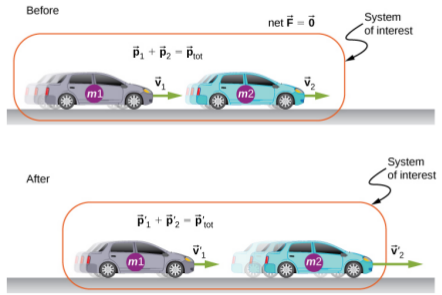
\includegraphics[width=0.7\textwidth]{figures/cars.png}
\caption{\label{fig:cars} The assumptions for momentum conservation.  (a) Which car exerts more force? (b) At which point are the cars accelerating?}
\end{figure}
\end{frame}

\begin{frame}{Conservation of Momentum}
\begin{figure}
\centering
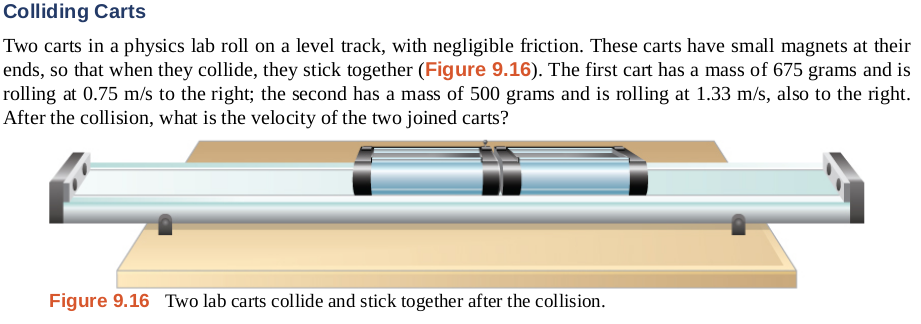
\includegraphics[width=0.8\textwidth]{figures/carts.png}
\caption{\label{fig:carts} The laboratory activity for today.}
\end{figure}
\small
\begin{itemize}
\item One cart still, other moving (magnet side)
\item One cart still, other moving (velcro side)
\item Both carts moving (magnet side)
\item Both carts moving (velcro side)
\end{itemize}
\end{frame}

\begin{frame}{Conservation of Momentum}
\small
\textbf{Test cases from lab:}
\begin{itemize}
\item One cart still, other moving (magnet side)
\item One cart still, other moving (velcro side)
\item Both carts moving (magnet side)
\item Both carts moving (velcro side)
\end{itemize}
\textbf{Answer the following questions:}
\begin{itemize}
\item In which of the above is the momentum conserved?
\item In which of the above is the kinetic energy conserved?
\item In which of the above is both the kinetic energy and momentum conserved?
\item In which of the above is the final kinetic energy zero?
\end{itemize}
\end{frame}

\begin{frame}{Conservation of Momentum}
\begin{figure}
\centering
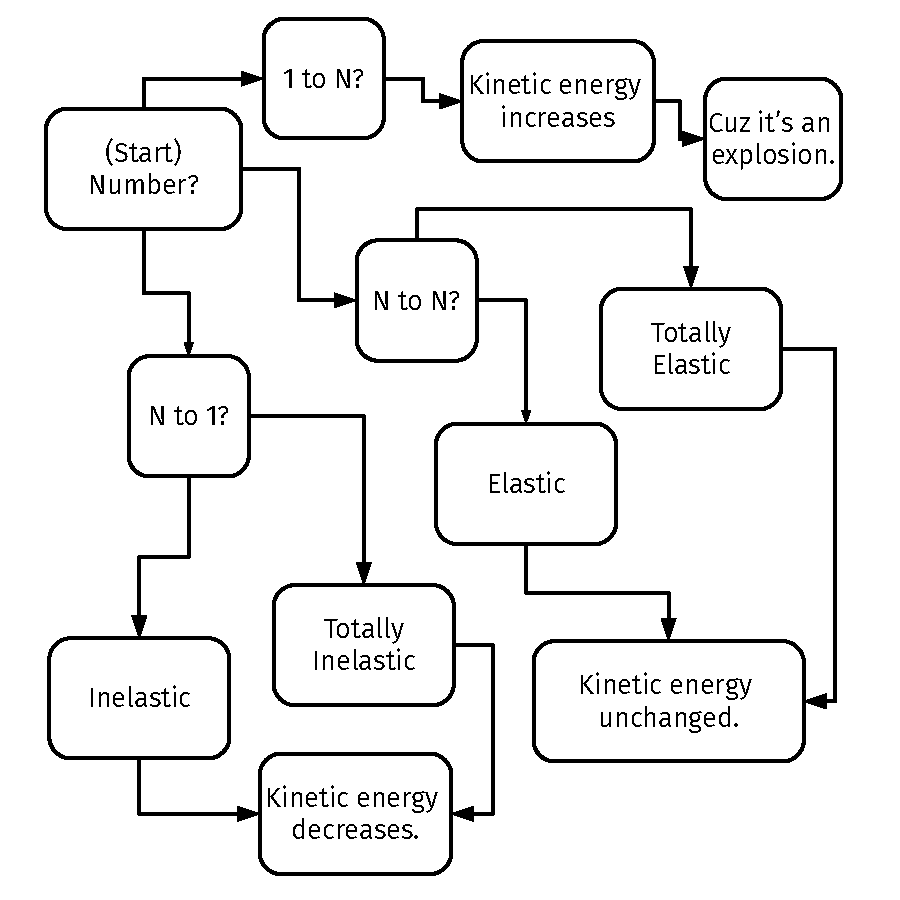
\includegraphics[width=0.6\textwidth]{figures/Flow.pdf}
\caption{\label{fig:flow} Classification of momentum interactions.}
\end{figure}
\end{frame}

\begin{frame}{Conservation of Momentum}
\textit{\alert{Special case of an} \textbf{explosion}...}
\url{https://www.youtube.com/watch?v=5zxVQBnmyDA}
\end{frame}

\begin{frame}{Conservation of Momentum}
\begin{figure}
\centering
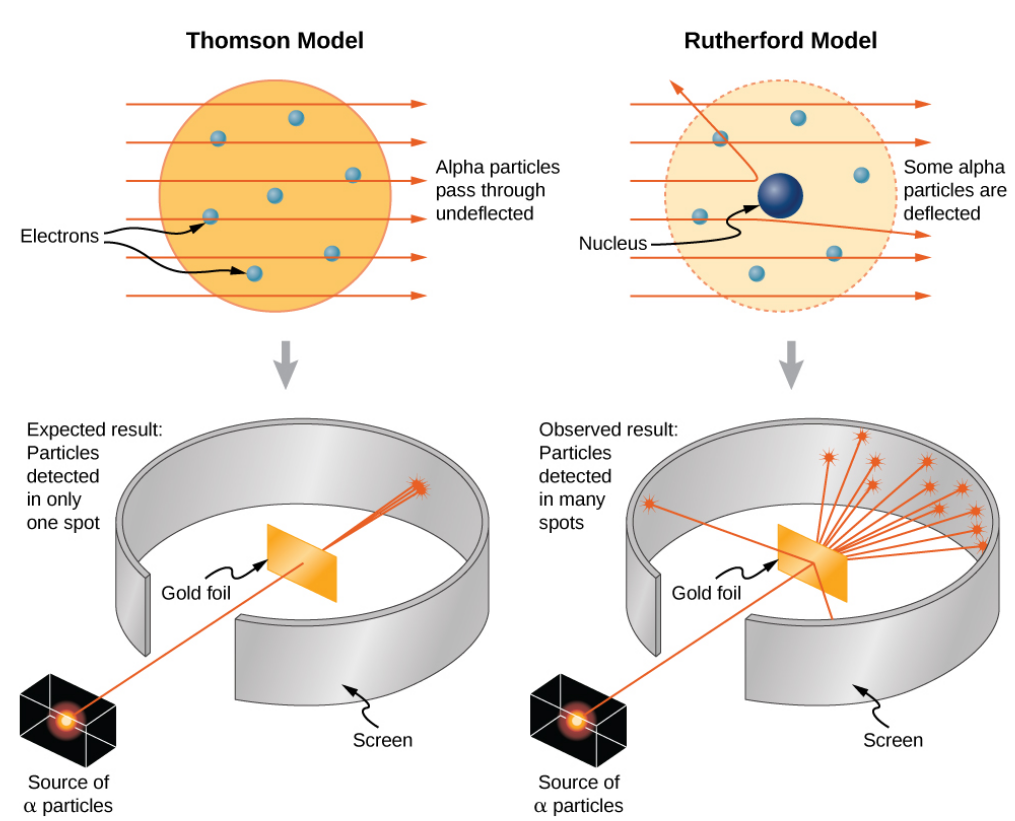
\includegraphics[width=0.75\textwidth]{figures/alpha.png}
\caption{\label{fig:alpha} Knowledge of the atom via momentum conservation! To understand the recoil energy, though, we have to understand the different possibilities: elastic or inelastic.}
\end{figure}
\end{frame}

\section{Elastic Collisions}

\begin{frame}{Elastic Collisions}
\begin{figure}
\centering
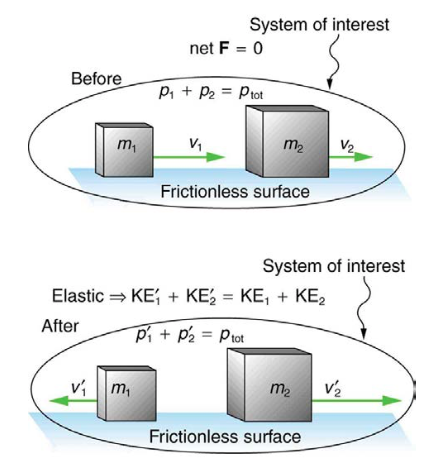
\includegraphics[width=0.55\textwidth]{figures/elastic.png}
\caption{\label{fig:elastic} \small Internal kinetic energy and momentum are conserved if the collision is \textit{elastic}.}
\end{figure}
\end{frame}

\begin{frame}{Elastic Collisions}
Suppose two objects undero an elastic collision.  Given the conditions below, find the quadratic equation for $v_{\rm 1}'$.
\begin{align}
m_{\rm 1} &= 0.5 kg \\
m_{\rm 2} &= 1.0 kg \\
v_{\rm 1} &= 2 m/s \\
v_{\rm 2} &= 0 m/s
\end{align}
\textit{\textbf{Solve in groups on boards.}}
\end{frame}

\begin{frame}{Elastic Collisions}
Suppose two objects undero an elastic collision.  Given the conditions below, find the quadratic equation for $v_{\rm 1}'$. \\ \vspace{0.5cm}
\textit{Answer:} $\frac{3}{2}v_{\rm 1}'^2 - 2v_{\rm 1}' - 2 = 0$ \\
\vspace{0.5cm}
Which root of this equation is correct, and why?
\end{frame}

\section{Inlastic Collisions}

\begin{frame}{Inlastic Collisions}
\begin{figure}
\centering
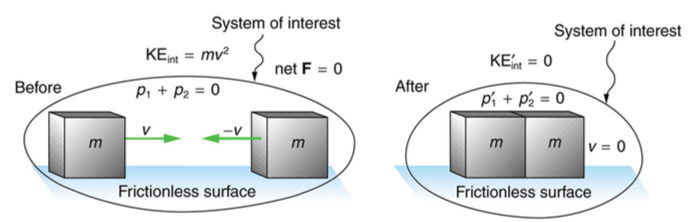
\includegraphics[width=0.9\textwidth]{figures/inelastic.png}
\caption{\label{fig:inelastic} Internal kinetic energy is not conserved, and momentum is conserved if the collision is \textit{inelastic}.}
\end{figure}
\end{frame}

\begin{frame}{Inlastic Collisions}
Suppose two objects undero an inelastic collision.  Given the conditions below,
\begin{align}
m_{\rm 1} &= 0.5 kg \\
m_{\rm 2} &= 1.0 kg \\
v_{\rm 1} &= 2 m/s \\
v_{\rm 2} &= 0 m/s
\end{align}
\textit{\textbf{Solve in groups on boards.}}
\end{frame}

\begin{frame}{Inelastic Collisions}
What is the right answer? \\ \vspace{0.5cm}
$v' = \frac{2}{3}$ m/s.  Should it be positive or negative?
\end{frame}

\section{Conclusion}

\section{Answers}

\begin{frame}{Answers}
\small
\begin{columns}[T]
\begin{column}{0.5\textwidth}
\begin{itemize}
\item $6\times 10^{43}$ J
\item The one with the small mass
\item The one with the large mass
\item $10^{-2}$ kg m/s
\item $10^{7}$ kg m/s
\item $-10^{7}$ N
\end{itemize}
\end{column}
\begin{column}{0.5\textwidth}
\begin{itemize}
\item The net external force is zero, and each mass is constant in time.
\end{itemize}
\end{column}
\end{columns}
\end{frame}

\end{document}
